\chapter{Database}

In this chapter we introduce the different methods we considered for a database representation and give reasons for final choice we made. Then we give a detailed description for our ER model.

%=======================================================================================
\section{Selection of the Database System}
For our database we considered NoSQL and SQL methods. We looked at different NoSQL solutions like MongoDB and CouchDB.
Since nobody who was responsible for the database had experience with NoSQL wo chose to stick with the SQL approach. We  wanted to build a slim system. Therefore we first started to use SQLite. At this time we still used Python in the backend. Later in our project Python became no possibility for us anymore so moved to PHP. This also meant that we would change our SQLite system to MySQL, because one of our group members already had experience with this combination. After considering different possibilities we finally arrived back at the standard solution for a database. The advantages fast, ... %TODO 
On the clumsy, often the solutions are too complex for uncomplicated problems...%TODO


%=======================================================================================
\section{ER-Model}
	For the database of our MyFood webpage service we created the following ER model.
	%Image from ER model, for a faster compilation time it is commented out
	%\begin{figure}[h!]
	%	\centering
	%		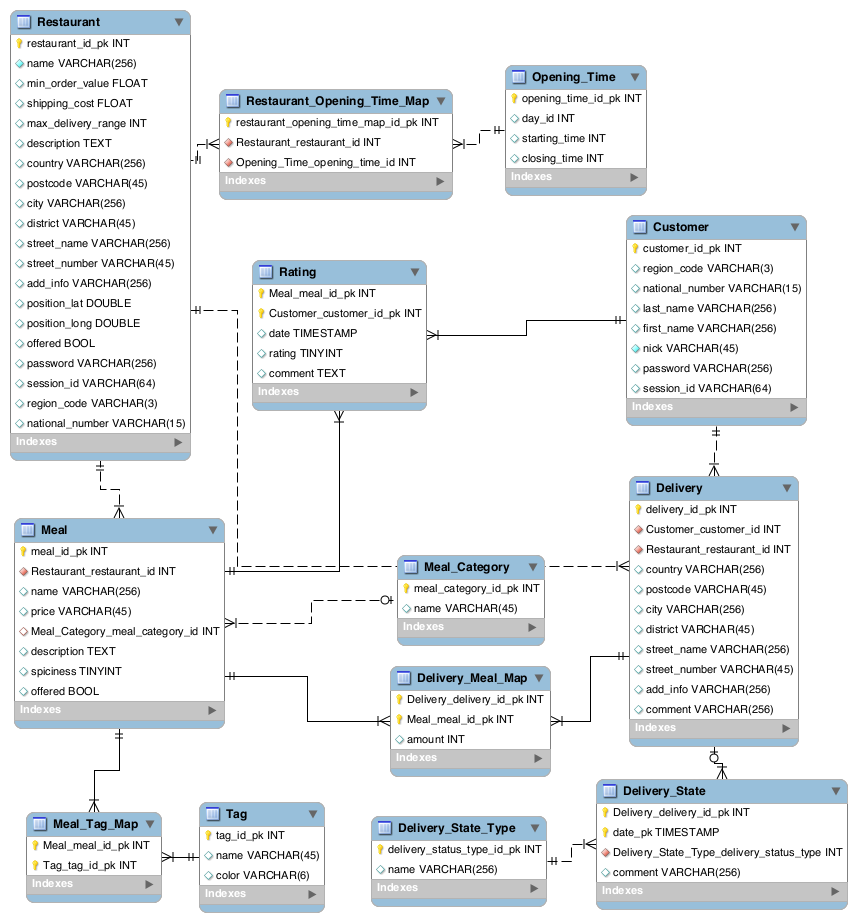
\includegraphics[scale=0.5]{content/graphics/er_model.png}
	%	\caption{ER model of our database.}
	%\end{figure}

	\subsection{Restaurant}
	The restaurant table represents the data of restaurant in real world.

	\setdescription{itemsep=5pt,parsep=0pt,leftmargin=0.5cm, style=sameline}
	\begin{description}
		\item[restaurant\_id\_pk: INT] This an automaticly generated surrogate key.
		\item[name: VARCHAR(256)] The name of the restaurant.
		\item[min\_order\_value: FLOAT] This value describes the minimum amount of value of a delivery so that a customer can submit a delivery.
	\end{description}

	\subsection{Delivery\_State}
	delivery state should be uniquely identified with the Delivery and time
